\section{Fault localization} \label{secFL}

%% what are the claims, what are we studying, why are we studying it


Spectrum-based fault localization (SBFL) is the most commonly studied dynamic
fault localization technique, and studies have shown that it is more effective
than other techniques such as Mutation-based fault
localization~\cite{mut-analysis} or dynamic program
slicing~\cite{zou2019empirical}. It is a key first step to characterizing the
\emph{fault space} in automatic program repair, narrowing it to a portion of the
program most likely to correspond to the fault.

Fundamentally, the core assumption underlying SBFL is that \emph{failing tests
  execute buggy portions of the code relatively more often than passing tests.}
Thus, if all failing tests execute a particular line of code, then that line of
code is highly suspicious.  SBFL techniques compute a suspiciousness by
measuring how often a line is executed by failing tests as compared to passing
tests. This suspiciousness score can be calculated a few different ways, but is
typically a linear combination of the passing and failing test coverage. One of
the oldest and commonly studied SBFL technique is Tarantula~\cite{tarantula}. In
Tarantula, the suspiciousness score for a line $s$ is calculated by:

$$\mathit{susp(s)} 
=\frac{\mathit{\%F(s)}}{\mathit{\%F(s)} + \mathit{\%P(s)}}$$

where  $\mathit{\%F(s)}$ and $\mathit{\%P(s)}$ are, respectively, the percentage of failing 
tests and passing tests that execute $s$. There are newer, more effective 
SBFL techniques that calculate this score differently, such as Ochiai~\cite{ochiai} and 
DStar~\cite{wong2013dstar}. Both of these were included in an empirical study 
comparing fault localization techniques and were found to localize a similar set of 
faults~\cite{zou2019empirical}.

Assigning a suspiciousness score to each line of code is well-suited to single
location repair. Indeed, the evaluation of most SBFL techniques asks exactly the
question of interest when considering a technique's suitability for
single-location repair: how often does a given technique correctly, highly rank
individual buggy lines of code?

Such evaluations, by and large, do not consider the implications of
suspiciousness scoring in a multi-location repair context.  Instead, evaluations
typically consider a technique ``successful'' if it identifies \emph{any} of a
set of changed lines as highly-ranked or likely-suspicious.  While appropriate
for the question being asked in such evaluations, this does not address
suitability for multi-location program repair.  Identifying one of several buggy
locations is generally inadequate in a context where multiple locations must be
modified. Thus, we ask the following research question:


\rqorinsight{How well do multiple tests cover the multiple locations
  implicated in bugs that require multi-location patches?}

To answer this research question, we investigate how well the SBFL assumption
applies to tests that identify bugs that require multi-location patches. We
focus especially on bugs that are associated with multiple failing tests: a bug
with only a single failing test trivially and equally implicates all the lines
that test executes.  If multiple tests cover the modified locations well, then
SBFL's core assumption holds and multi-location repair can expect to effectively
make use of the off-the-shelf ranking these techniques currently provide
(indeed, this has been tried~\cite{angelix}). If not---that is, if multiple
tests exercise \emph{different} portions of the buggy code---SBFL off-the-shelf
will by definition be less effective in guiding APR to correctly modifying
multiple buggy locations at once.

Therefore, for these bugs, do the different failing tests cover exactly the same
patch locations, exactly disjoint patch locations, or some combination?

\paragraph{Methodology}

Between both datasets, there are 92 total bugs that both require multi-location
patches and contain multiple failing tests: 59 in Defects4J, and 33 in
Bears. \todo{There is one bug in bears that I couldn't get coverage for through
  my tool or by inspection; what do I do about that?  (It's currently
  counted in the 92 bugs but not in the graphs)}
For each of these bugs, we used JaCoCo\footnote{https://www.eclemma.org/jacoco/}
to determine which of the patched locations were executed (at least once) by
each failing test. Using this coverage data, we categorized each bug as follows:
\begin{itemize}
\item \emph{disjoint} bugs are those for which no patch location is covered by all
failing tests.  Inutitively, these are the bugs for which the core SBFL
assumption is violated.
\item \emph{overlap} bugs are those for which some faulty locations are covered
by all failing tests, but some are only covered by a subset of the failing
tests. These bugs also violate the core assumption of SBFL, albeit to a lesser
extent.
\item \emph{identical} bugs are those for which all tests cover the exact same
  set of patch locations.
\end{itemize}


\begin{figure}
	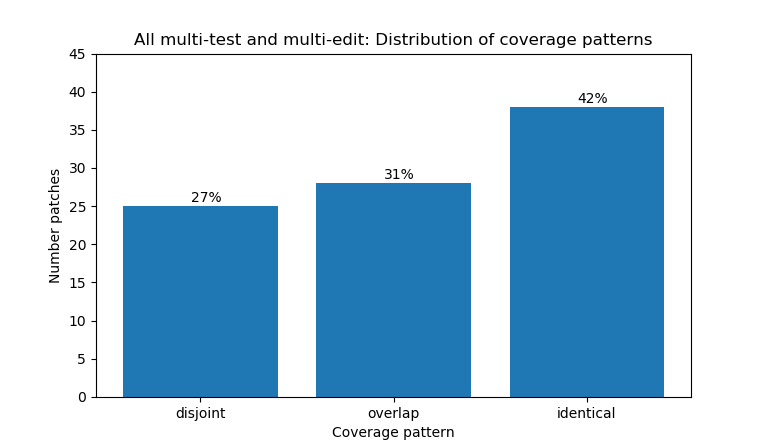
\includegraphics[width=\linewidth]{img/coverage-all.png}
	\caption{Distribution of coverage patterns for bugs with multiple failing
      tests that are repaired with multi-location patches in Bears and Defects4J.}
	\label{fig:coverage-all}
\end{figure}


\begin{figure}
	\begin{subfigure}{\linewidth}
		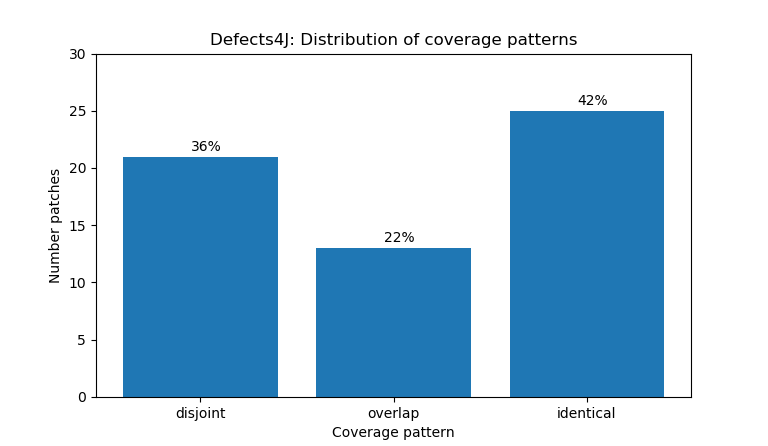
\includegraphics[width=\linewidth]{img/coverage-d4j.png}
		\caption{Distribution of coverage patterns for Defects4J.}
	\end{subfigure}
	\begin{subfigure}{\linewidth}
		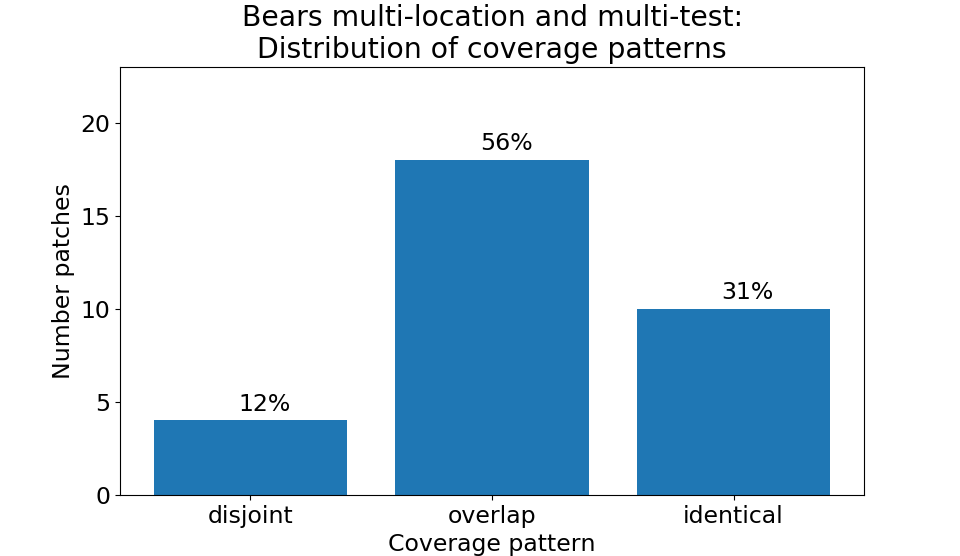
\includegraphics[width=\linewidth]{img/coverage-bears.png}
		\caption{Distribution of coverage patterns for Defects4J.}
	\end{subfigure}
	\caption{Distribution of coverage patterns divided by dataset,
          indicating significant differences between the multi-location bugs in
          Bears and Defects4J.}
	\label{fig:coverage-datasets}
\end{figure}

\paragraph{Results}
Figure~\ref{fig:coverage-all} shows results for the overall distribution,
combining the bugs in both datasets. 27\%
of the bugs were fully disjoint.  Thus, for a significant portion of multi-location bugs,
the failing tests do not all execute any of the buggy code in common.  
In addition, another 31\% were classified as \emph{overlap}: only some of the
buggy locations were executed by all failing tests. In all, over half of 
the bugs that were both multi-location and multi-test contained chunks that were 
not executed by all failing test cases.

\todo{Ooooooh I have a question about results we can't ansewr in 24 hours but
  can answer in refinement to this work: do those failing tests have \emph{any}
  overlap, as in, on the \emph{non-buggy} code?  Because if so, that's
  \emph{much} worse for FL of multi-edit bugs.}

Note, however, that the behavior varies considerably by dataset;
Figure~\ref{fig:coverage-datasets} shows results.  Defects4J and 
Bears have very different distributions with respect to the 
disjoint and same categories. In Defects4J, 36\% of bugs are \emph{disjoint} and 
22\% are \emph{overlap}; in Bears, the proportions are 12\% and 47\%, respectively.
We hypothesize that this may be due to differences in how the two  
datasets were selected and minimized: Defects4J is a dataset of minimized and curated 
bugs, while the bugs in Bears are scraped directly from the
commits. The Defects4J dataset specifically enforces a requirement that the patches in the 
dataset be isolated, i.e., not containing any refactorings or new features, to improve the 
usability of the dataset. The authors specifically chose patches that met this requirement, 
and in some cases, isolated the bug themselves, manually~\cite{defects4j}. In contrast, the 
only requirements for inclusion of bugs in Bears is that it must be reproducible and 
the patch must be written by a human. In addition, Bears was designed to be evolvable 
and relatively easily expanded, which is at odds with manual inspection and isolation of 
bugs~\cite{bears}.
Given that these two datasets were designed with different values and demonstrate very 
different behavior, these findings highlight the importance of using diverse datasets. 
\todo{I don't actually know of work that argues that we should be using diverse dataset ? 
But maybe Claire you have an idea.}

\todo{below is original todo, which I've tried to address:}
\todo{references to the original papers in citations would be good,
  here.}  \todo{1--2 more sentences...what's the implication?  Something like
  ``this supports recent work arguing for a diversity of datasets and
  identifying the risk of overfitting to our datasets.''  But also, as
  discussed, I think this may not be a terrible thing about Defects4J....like,
  maybe the minimization means that D4J is more focused on the edits actually
  necessary to fix a bug, and that the results on D4J are subsequently more
  indicative in terms of what fault localization needs to do to work for
  multi-edit repair.  I'm comfortable with that level of speculation, but we
  need to spell it out here (and we are not currently spelling it out).  If we
  do, then I'm comfortable with the claim in the concluding/next paragraph.}

SBFL assumes that faulty locations are executed more often by identifying 
or failing test cases and is not designed to find faults like these. Since SBFL 
is the most common fault localization technique in APR, most APR techniques 
are not well suited to fix a majority of these multi-location and multi-test 
bugs.



%\section{Symptoms}

We want to study symptoms in the context of fault localization. We define symptoms as the output given in failing test cases. In Java, most of these symptoms will be exceptions and their accompanying error message. Since most program repair is based off of failing tests, we want to see if those symptoms exhibited in those tests can correlate to type of repair.

For this paper, we specifically wanted to look at whether symptoms correlated with whether a bug could be fixed in a single location or multiple locations. If we can classify which bugs are single edit or multi edit, we can choose fault localization or patch generation techniques that are more suited.

We looked at all symptoms for all bugs in Defects4J and Bears, and categorized them based on whether they were one of the identified multi-chunk bugs or not. Then we fit the data to a linear regression model to see if there were statistically significant differences between the type of symptoms for multi edit and single edit bugs.

In order to find statistical significance, we needed to categorize the symptoms in big enough categories. We experimented with three groupings:

\begin{enumerate}
	\item Group all exceptions together except for assertion exceptions and exceptions for which a message indicates some sort of assertion (in our case, we simply looked for the keyword "expected"). We grouped the assertions into a few different types: 
	\begin{itemize}
		\item \lstinline{assert_null} is when the assertion is either expecting null, or got null when it wasn't expecting it.
		\item \lstinline{assert_int} is when the failing assertion was expecting a particular int value.
		\item \lstinline{assert_float} is the same as above, but for floats.
		\item \lstinline{assert_obj_arr_date} is when the assertion is expecting an object address, array of objects, or date object/date string. These are grouped together as commonly found but more complex assertions.
		\item \lstinline{error_expected} is when the failing test expected an exception, error, or warning.
		\item \lstinline{timeout} is when a Junit test times out, but also includes errors like stack overflows or out of memory exceptions.
		\item \lstinline{other_assert} for any other assertion that I couldn't easily categorize or parse. The large bulk of bugs in this category are bugs that had no error message at all; it simply failed with an \lstinline{AssertionError} or \lstinline{StackOverflow}.
		\item \lstinline{other}: all non-assertion exceptions.
	\end{itemize}
	\item Grouping symptoms together in an ad hoc way \todo{sell it better.}
	\begin{itemize}
		\item \lstinline{assert_prim}: assertions that compare to a Java primitive, such as int, float, or boolean.
		\item \lstinline{assert_null}: either expected or actual is null
		\item \lstinline{other_assert}: Asserting to anything that's not clearly a primitive or null.
		\item \lstinline{access}: all the bugs pertaining to wrongfully accessing or invoking certain fields or methods, or problems with classpath.
		\item \lstinline{null_pointer}: null pointer exceptions.
		\item \lstinline{timeout}: when a Junit test times out, but also includes errors like stack overflows or out of memory exceptions.
		\item \lstinline{parsing}: Anything related to parsing, serialization, or type conversion.
		\item \lstinline{other}: everything else
	\end{itemize}
	\item This last grouping is an even coarser version of the previous grouping.
	\begin{itemize}
		\item \lstinline{assert_equal}: Any assertion in which the test expected one value but got another
		\item \lstinline{other_assert}: any other assertion
		\item \lstinline{access}: all the bugs pertaining to wrongfully accessing or invoking certain fields or methods, or problems with classpath.
		\item \lstinline{null_pointer}: null pointer exceptions.
		\item \lstinline{parsing}: Anything related to parsing, serialization, or type conversion.
		\item \lstinline{other}: everything else
	\end{itemize}
\end{enumerate}

\todo{raw data from bogdan:}

assert only
\begin{lstlisting}
Call:
glm(formula = multi ~ assert_obj_arr_date + assert_int + assert_float + 
error_expected + timeout + assert_null + other_assert + other, 
family = "binomial", data = symptoms)Deviance Residuals: 
Min       1Q   Median       3Q      Max  
-1.2466  -0.5686  -0.4691  -0.4394   2.2880  Coefficients:
Estimate Std. Error z value Pr(>|z|)    
(Intercept)             -2.37550    0.38061  -6.241 4.34e-10 ***
assert_obj_arr_dateTRUE  1.24082    0.50907   2.437   0.0148 *  
assert_intTRUE           0.08619    0.45621   0.189   0.8502    
assert_floatTRUE         2.31273    0.48580   4.761 1.93e-06 ***
error_expectedTRUE       0.36735    0.53943   0.681   0.4959    
timeoutTRUE              0.99295    0.65378   1.519   0.1288    
assert_nullTRUE         -0.16611    0.58071  -0.286   0.7748    
other_assertTRUE         0.22402    0.36136   0.620   0.5353    
otherTRUE                0.63507    0.38201   1.662   0.0964 .  
---
Signif. codes:  0 '***' 0.001 '**' 0.01 '*' 0.05 '.' 0.1 ‘ ’ 1(Dispersion parameter for binomial family taken to be 1)    Null deviance: 546.49  on 645  degrees of freedom
Residual deviance: 510.11  on 637  degrees of freedom
AIC: 528.11Number of Fisher Scoring iterations: 5
\end{lstlisting}

grouping 1
\begin{lstlisting}
Call:
glm(formula = multi ~ access + assert_prim + null_pointer + timeout + 
assert_null + parsing + other_assert + other, family = "binomial", 
data = symptoms)Deviance Residuals: 
Min       1Q   Median       3Q      Max  
-0.9771  -0.6792  -0.5070  -0.4031   2.5944  Coefficients:
Estimate Std. Error z value Pr(>|z|)    
(Intercept)      -1.94778    0.36198  -5.381 7.41e-08 ***
accessTRUE        0.62756    0.41197   1.523   0.1277    
assert_primTRUE   0.81567    0.36223   2.252   0.0243 *  
null_pointerTRUE  0.32833    0.52496   0.625   0.5317    
timeoutTRUE       0.64782    0.63743   1.016   0.3095    
assert_nullTRUE  -0.52160    0.57971  -0.900   0.3682    
parsingTRUE       0.64081    0.50451   1.270   0.2040    
other_assertTRUE -0.03905    0.34777  -0.112   0.9106    
otherTRUE        -1.38263    0.76326  -1.811   0.0701 .  
---
Signif. codes:  0 '***' 0.001 '**' 0.01 '*' 0.05 '.' 0.1 ‘ ’ 1(Dispersion parameter for binomial family taken to be 1)    Null deviance: 546.49  on 645  degrees of freedom
Residual deviance: 523.84  on 637  degrees of freedom
AIC: 541.84Number of Fisher Scoring iterations: 5
\end{lstlisting}

grouping 2
\begin{lstlisting}
Call:
glm(formula = multi ~ assert_equal + access + null_pointer + 
parsing + other_assert + other, family = "binomial", data = symptoms)Deviance Residuals: 
Min       1Q   Median       3Q      Max  
-0.9390  -0.6809  -0.4377  -0.4377   2.2494  Coefficients:
Estimate Std. Error z value Pr(>|z|)    
(Intercept)       -2.0821     0.3470  -6.001 1.96e-09 ***
assert_equalTRUE   0.7532     0.3333   2.260   0.0238 *  
accessTRUE         0.7259     0.3979   1.824   0.0681 .  
null_pointerTRUE   0.4338     0.5131   0.845   0.3979    
parsingTRUE        0.7385     0.4976   1.484   0.1378    
other_assertTRUE  -0.2150     0.3223  -0.667   0.5048    
otherTRUE         -0.3646     0.5068  -0.719   0.4719    
---
Signif. codes:  0 '***' 0.001 '**' 0.01 '*' 0.05 '.' 0.1 ‘ ’ 1(Dispersion parameter for binomial family taken to be 1)    Null deviance: 546.49  on 645  degrees of freedom
Residual deviance: 527.48  on 639  degrees of freedom
AIC: 541.48Number of Fisher Scoring iterations: 5
\end{lstlisting}

In assert only, \lstinline{assert_float} correlates strongly with multiedit bugs. However, all the instances of \lstinline{assert_float} as a symptom occur in the Math package for Defects4J, and they all somehow to be multichunk. The sampling of \lstinline{assert_float} can be seenin the other two groupings as well, where \lstinline{asset_prim} and \lstinline{assert_equal}, both of which subsume \lstinline{assert_float}, are both more likey to be multi-edit.  \todo{take out math, redo analysis?}



